\documentclass[12pt, letterpaper]{article}

\usepackage{graphicx}
\graphicspath{ {images/} }
\usepackage[letterpaper, margin=1in]{geometry}
\usepackage{indentfirst}
\usepackage{secdot}
%\usepackage[toc,page]{appendix}
\usepackage{tocloft}
\usepackage{tabularx}
%\renewcommand{\baselinestretch}{1.9}
\usepackage{setspace}
\usepackage{float}
\doublespacing

\newcommand{\companyname}{Veg-To-Go}

\begin{document}


\includegraphics[width=\textwidth]{VegToGoLogo}

\newpage{}

\title{\companyname{},\textsuperscript{\texttrademark} Food Truck\\ Marketing Plan}
\author{Zach Pratt}
\maketitle

\newpage

\renewcommand\contentsname{Table of Contents}
\renewcommand{\cftsecleader}{\cftdotfill{\cftdotsep}}
\tableofcontents

\newpage

\section{Executive Summary}
Veg-To-Go is an upcoming mobile food venue serving a hearty and filling menu of plant based, animal and animal product free comfort food.  While the trend of food trucks, tents, and truck bed barbeques is already prominent in Fort Wayne, there is still a lack in these existing businesses of concern for the ethics of food.

Veg-To-Go hopes to provide wholesome and filling plates of flavorful and saucy food at a bigger price-to-ounce ratio, ultimately giving customers more savory food for their dollar.  This plan will show that this results in a bigger profit margin, saving the company money by eliminating expensive animal products and using simple frozen and fresh ingredients combined with proven methods of boosting savories using spices and herbs.

Building on this mission to completely satisfy Fort Wayne street food customers with cheap, generous, and healthy food, Veg-To-Go begins to incrementally building its customer base.  The company starts by purchasing a minimal setup of a small flattop grill and source its frozen and dry ingredients from local warehouse and bulk sections. Produce is be purchased locally and fresh when possible.  The company attends weekly farmers markets and set up outside bars throughout the week when possible.  After an initial trial phase and the establishment of a solid customer base, the company purchases a dedicated food truck or other mobile venue to expand its existing business.

\section{Situation Analysis}
This situation analysis demonstrates the current state of \companyname{} by examining the business environment through a SWOT analysis and detailed examination of the industry, competitors, company, and consumers.

\subsection{SWOT Analysis}
Figure \ref{SWOT} shows the factors affecting the market opportunities for \companyname{}.  This table highlights the efforts by the company to prepare to enter the local market.

\begin{figure}[H]
	\label{SWOT}
	\caption{SWOT analysis for \companyname{}}
	\centering
	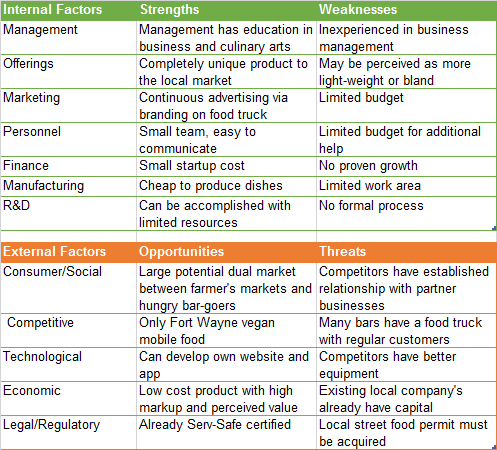
\includegraphics{SWOT}
\end{figure}

\subsection{Industry Analysis: Trends in Mobile Food Venues}
According the National Restaurant Association, the annual US food truck revenue is 2.7 billion dollars annually and rising. \cite{ibis1} With this kind of opportunity, it comes as no surprise
that many local entrepreneurs have begun to emerge. According to the Fort Wayne Food Truck association, there are over 51 food trucks, 14 organized under the association and 37 unorganized or non-affiliated trucks. \cite{fwfta}

\subsection{Competitor Analysis: Local Food Trucks}
Of the 51 food trucks in Fort Wayne, none are oriented toward health, sustainability, or a plant-based lifestyle. \cite{fwfta2} The existing local trucks vary in level of activity and success.  The top three most successful food trucks in Fort Wayne are Ragin' Cajun, Affine, and Bravas. \cite{fwfta2} Of those three, only Bravas offers a plant-based item: a hot dog with traditional toppings.  Affine attempts a farm-to-fork concept but this is mainly evident in their meat offerings.

A non-food-truck plant-based restaurant does exist in Fort Wayne: Loving Cafe. They offer everything from raw food to sandwiches that employ fake meat, to sodas and dessert.  Loving Cafe has enjoyed much success and are expanding their kitchen staff, but are family owned/operated and have no plans to expand to new markets in town.

\subsection{Customer Analysis}
The primary target audience for Veg-To-Go is 18-35 years old male and female Fort Wayne residents with individual income under \$55,000 per year.  The secondary market is families out on family outings at sporting events or farmer's markets.
\subsubsection{Customer Characteristics}
The primary market is composed of nightlife: individuals who are out late at night at bars looking for filling food to satisfy spontaneous appetites. They want something that tastes rich and savory and also fills them but don't want to spend too much money. They care about the immediate access and are willing to pay in cash for the convenience. The secondary audience is families who are out at farmer's markets or shopping during the week.  These individuals are the main target promotional market during the first year of operation.
The second and third year sees the expansion of promotion to families.  These families are looking for a wholesome meal that can be shared and enjoyed together. They are looking for the convenience of location as well as health. 
\subsubsection{Health and Nutrition Concerns}
Although the first market of 18-35 year olds after 9pm are traditionally seen as primarily looking for flavor in the product, the company plans on targeting this ever growing market by appealing to their desire for food to fuel their fun.  The energy gained from the vegetables and rice are emphasized.  In addition the main savory component in each sauce, nutritional yeast, which adds a "meaty" quality to the dish, contains 480\% daily value of B6 per serving, and 130\% of B12. \cite{yeast} This makes \companyname{} food energy boosting and considerably flavorful, which is a huge draw for late-nighters.

The secondary market of families is targeted with the mixture of vegetables and the inherent health benefits from consuming them.  Mothers and Fathers are looking for something healthy and quick, and \companyname{}'s food satisfies both of these needs. Farmer's markets serve as both an outlet for the company to provide warm meals and also a promotional platform to showcase the local fare. This has a positive impact while catering to the perceived need of the farmer's market demographic to eat healthy and local.

\section{Market-Product Focus}
The following describes the three-year marketing objectives of \companyname{}, detailing the target markets, competitive advantages, and product positioning in the local market.
\subsection{Marketing and Product Objectives}
\companyname's{} marketing objectives during the first three years are threefold.  Make a strong opening statement, establish itself as the premier venue for on-the-go plant-based food with its primary and secondary target markets, and maintain strong relationships with it's partners. 

\textbf{\emph{Strong debut.}} Firstly, the company aims to make a strong debut in the local food truck market.  This is accomplished by means of setting a strong schedule of appearances with key partner venues in the area.

\textbf{\emph{Product Positioning.}} \companyname{} aims to be the premiere plant-based food venue in Fort Wayne.  By offering consistent and widely appealing food the company does not simply target the vegan or health-conscious demographics, but looks first to the younger population and rely on grassroots advertising in addition to its own promotional efforts.

\textbf{\emph{Partner Relations.}} \companyname{} utilizes its on-line presence and strong understanding of the intersection of service marketing and technology to create a partner network and online promotional ecosystem that provides mutual benefits. These established relationships are key to the survival of \companyname{} and fostering them is a priority for the company.

\subsubsection{Target Markets}
Maecenas laoreet, ante sit amet malesuada mattis, sem libero egestas magna, ut commodo velit quam ut magna. Phasellus in eros at mi gravida rutrum. Etiam volutpat imperdiet malesuada. Vestibulum consequat ipsum pharetra, mattis turpis ut, dignissim diam. Curabitur et egestas sem. Mauris eu dui arcu. Sed quis nisi purus. Sed vitae porttitor ligula. Donec interdum metus ac turpis luctus gravida. In ultrices sem vitae magna finibus, vel condimentum tortor volutpat. Aliquam erat volutpat. Maecenas laoreet lectus ac purus luctus, nec accumsan risus tempor. Phasellus turpis massa, varius vitae massa nec, elementum aliquet libero. Praesent egestas feugiat massa sed tincidunt. Fusce pulvinar aliquet velit, et vulputate ligula aliquam vel. Donec at suscipit quam.

\subsubsection{Points of Difference}
\companyname{} has three key differentiators from its competition in the local 18-35 nighttime market:

\begin{itemize}
	\item \emph{Portion Size.}  \companyname{} offers larger portion sizes and more food per ounce than competitors for one simple reason: ingredient cost.  Vegetables and rice serves as the main components in the company's product, and on average vegetables cost a tenth of what meat does. \cite{costs}
	\item \emph{Variety.} \companyname{} fills the need in the illusive spontaneous nightlife for variety by offering food from five different countries.  Each visit to \companyname{} can provide an experience that is completely different in flavor but the same in quality and flavor.
	\item \emph{Sustainability.} According to a poll trying to identify millennial's top priorities, two-thirds of respondents said they would pay more for a product from a company that focused on sustainability. \cite{millennials} This puts \companyname{} in a unique position as no other mobile food venues in Fort Wayne emphasize sustainability.
\end{itemize}

\subsubsection{Positioning}
\companyname{} effortlessly fills a need in it's primary and secondary markets by simultaneously being healthy and hearty.  Current offerings fill neither of these needs as portion sizes and price per ounce tend to be greater than in non-mobile counterparts. \companyname{} avoids the need to charge more per ounce by saving money on ingredient costs.  Not only this, but \companyname{} is just as convenient and present as the competition.

\section{Marketing Program Strategy and Tactics}
\subsection{Product Strategy}
\textbf{\emph{Fresh.}} Local produce is purchased when possible, resulting in a seasonal and varied product. Many of these vegetables are cooked and served at the same farmer's market they were purchased at from partners on the same day or week.

\textbf{\emph{Fast.}} Components are assembled off-site in advance where applicable, saving assembly time and improving delivery time and order fulfillment on-site. Examples include: rice cooked for the day, sauces prepped and stored, and vegetables cut in advance, preferably packaged in weighed portions for each dish. Dishes are served on sustainable and durable disposable dishware.

\textbf{\emph{Flavorful.}} Bulk herbs and spices is purchased through local and online sources, allowing a predictable and constant flavor in each dish.  The dishes  all contain the same vegetables and rice, with the flavor being dictated by the sauce used.  The flavors are: Indian, Thai, Italian, Chinese, and Mexican. Side dish offering vary slightly but almost always include Fried Potatoes, Cole Slaw (with Simply Mayo\textregistered{} vegan mayonnaise) and "Mac and Cheez" with a vegan cheese sauce and veggie of the day.
\subsection{Price Strategy}
All entree dishes are equally priced at \$8 a plate, and sides at \$4 per serving. Entrees contain between 12 and 16 ounces of food at \$.50 an ounce. The ingredients for each dish cost at most \$.15 an ounce, with the bulk of the meal consisting of rice (approximately \$.03 an ounce \cite{costs}) and the rest mixed vegetables (\$.10 and ounce) with dried herbs and spices (\$.02 an ounce), yielding approximately a desirable 3 times markup. A similar markup is applied to the sides.  These prices remain constant the first three years.
\subsection{Promotion Strategy}
Promotion is to be done as the budget allows, using roughly 2\% of quarterly revenue and consists of food giveaways and graphical posters strategically placed in bars and at schools.  Customers may also check in through Facebook, Google+ or the Veg-To-Go mobile app to get 10\% off their meal.

Promotion the first year focuses heavily on the Mexican and Chinese dishes at first (see Figure \ref{products}), featuring the potatoes as a side. After the first year, the Italian entree is added to the promotional mix.

The first target market consists of adults 18-35 at nighttime venues and primarily appeals to a need to eat a filling meal while out with friends and secondarily appeal to a sense of doing good for the environment by eating sustainably.

Sign-age and graphical promotion begin to expand the second year to target families at daytime venues.  Advertising during the day incorporates imagery and phrasing to reflect eating hearty and healthy in the context of a family outing.
\subsection{Place (Distribution) Strategy}
Relationships are established with local bars, nightlife locations, and farmer's markets during the first year.  Some of the promotional budget is used to provide meal trade and incentives to establish rapport with these partner businesses.  In addition, advertising may be offering through the company's mobile app and social media outlets for partners, which reduces some cost in forming these alliances.  Nightclub parking lots, bars, and other popular after 9pm spots are targeted.

The second and third year is about maintaining a consistent presence and expanding to the company's secondary target market (families) by offering free 1/2 size meals for children 12 and under at daytime venues.  These venues include the Fort Wayne Farmer's Market and other farmers markets, Indiana Purdue University Fort Wayne, and Fort Wayne Tincaps Games.

\section{Financial Projections}
\subsection{Three-Year Projections}

\begin{figure}[H]
	\caption{Sales and Expenses for \companyname{}}
	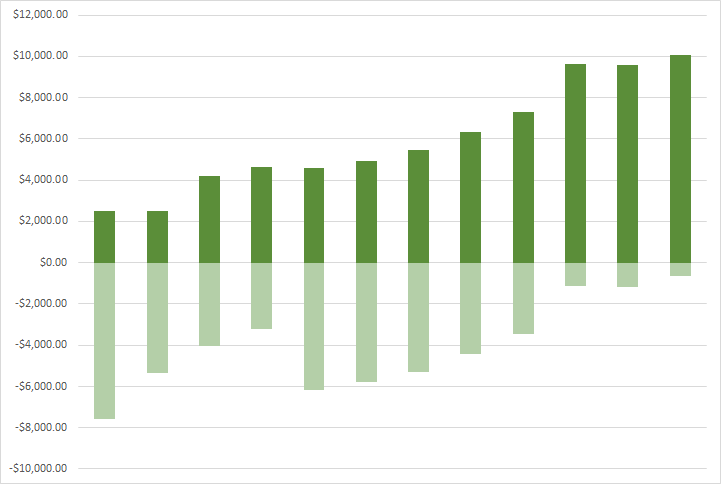
\includegraphics[width=\textwidth]{SalesAndExpenses}
\end{figure}

\begin{figure}[H]
	\label{products}
	\caption{Three Year Projected Sales for \companyname{}}
	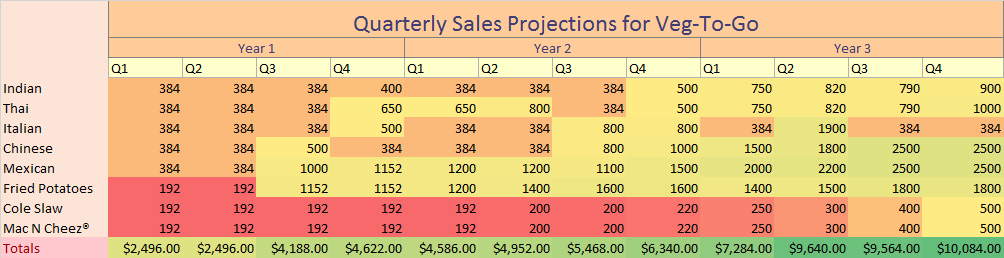
\includegraphics[width=\textwidth]{SalesNumbers}
\end{figure}

\begin{figure}[H]
	\caption{Three Year Projected Expenses for \companyname{}}
	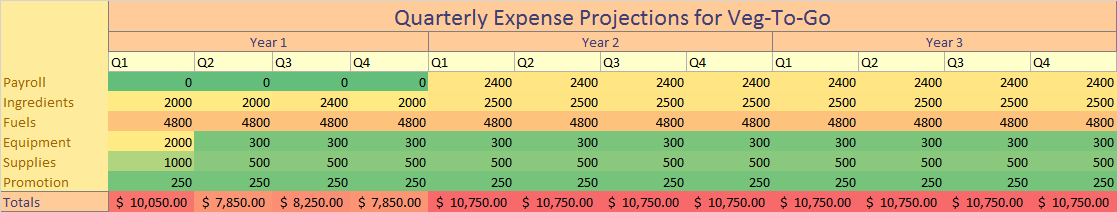
\includegraphics[width=\textwidth]{ExpensesNumbers}
\end{figure}

\begin{figure}[H]
	\caption{Total 3-Year Net Profit Projection (Numbers) for \companyname{}}
	
\includegraphics[width=\textwidth]{TotalProfitNumbers}
\end{figure}

\begin{figure}[H]
	\caption{Total 3-Year Net Profit Projection (Visual) for \companyname{}}
	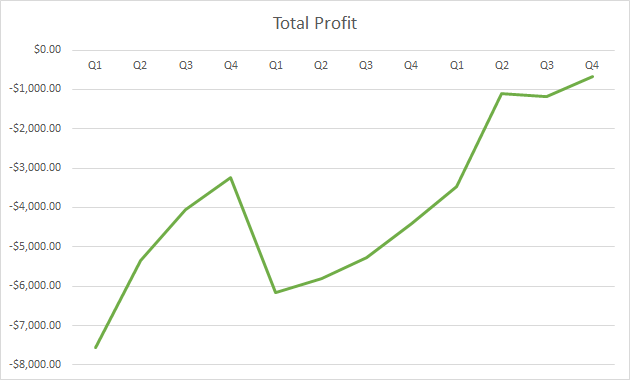
\includegraphics[width=\textwidth]{TotalProfit}
\end{figure}

\section{Implementation Plan}
The company initially purchases a graphical tent under which the food is cooked and served truck-side.  A single induction burner serves as the heating elements for pre-prepared, fresh ingredients.  The dishes mainly consist of a sauce that dictates the cuisine, combined with veggies and served over white rice.  The setup and costs are kept to a minimum, but the flavor is boosted using lightweight dried and fresh herbs and spices and international inspiration.

The company is operated by a single owner, and after the first year an employee is hired for 5 hours a day at \$10 and hour.

\section{Evaluation}
Lorem ipsum dolor sit amet, consectetur adipiscing elit. Aenean fringilla sem et suscipit dapibus. Quisque a pulvinar mi, nec aliquet metus. Curabitur hendrerit porttitor purus. Phasellus a est nec ante pellentesque maximus. Mauris commodo enim risus, eget porttitor odio pharetra ac. Nullam elementum congue enim eget facilisis. Mauris lacus urna, bibendum ut venenatis fringilla, varius ac tellus. Curabitur venenatis rutrum nunc. Mauris in porttitor justo. Phasellus in vulputate eros. Mauris maximus diam eu tortor mattis, sed imperdiet dui rhoncus. Morbi ultrices maximus metus sed eleifend. Maecenas vestibulum in nibh efficitur imperdiet. Curabitur finibus tempor vehicula. Praesent pellentesque id justo eget blandit. Maecenas id odio nulla.

Sed vel sagittis nisi. Donec auctor eu est sed maximus. Aenean pharetra tincidunt ipsum, at rhoncus ipsum ullamcorper at. Nulla fringilla ligula nec risus maximus, ac gravida lorem pellentesque. Fusce vehicula malesuada fringilla. Nunc iaculis, lectus non faucibus dapibus, elit sapien hendrerit ipsum, id vehicula odio lacus ornare neque. Nullam in est pellentesque, euismod turpis et, ultrices ante.

Maecenas laoreet, ante sit amet malesuada mattis, sem libero egestas magna, ut commodo velit quam ut magna. Phasellus in eros at mi gravida rutrum. Etiam volutpat imperdiet malesuada. Vestibulum consequat ipsum pharetra, mattis turpis ut, dignissim diam. Curabitur et egestas sem. Mauris eu dui arcu. Sed quis nisi purus. Sed vitae porttitor ligula. Donec interdum metus ac turpis luctus gravida. In ultrices sem vitae magna finibus, vel condimentum tortor volutpat. Aliquam erat volutpat. Maecenas laoreet lectus ac purus luctus, nec accumsan risus tempor. Phasellus turpis massa, varius vitae massa nec, elementum aliquet libero. Praesent egestas feugiat massa sed tincidunt. Fusce pulvinar aliquet velit, et vulputate ligula aliquam vel. Donec at suscipit quam.

Suspendisse semper lectus in nulla luctus semper. Praesent a fermentum ipsum. Fusce eget cursus mauris, id finibus lectus. Ut erat velit, finibus molestie porttitor sit amet, tincidunt ac magna. Vestibulum a dui dolor. In ut ipsum est. Mauris dui felis, elementum et mauris quis, eleifend gravida enim. Fusce justo est, varius quis eleifend lacinia, semper ac enim. Curabitur lobortis lorem quis purus facilisis egestas. Praesent non leo non enim facilisis imperdiet.

Proin feugiat, augue vitae sagittis ullamcorper, diam sem tincidunt lectus, non elementum dolor nisl a tortor. Duis sed diam tincidunt dui pharetra finibus vitae nec tellus. Etiam sed nibh commodo, consectetur enim et, tempor lacus. Fusce eu porttitor tellus. Aenean egestas mi eu ultrices fermentum. Duis euismod vulputate massa nec dignissim. Aenean viverra at velit quis viverra.

\newpage

\begin{thebibliography}{9}


	\bibitem{costs}
		Average Retail Food and Energy Prices, U.S. and Midwest Region. (n.d.). Retrieved November 14, 2015, from http://www.bls.gov/regions/mid-atlantic/data/AverageRetailFoodAndEnergyPrices\_USandMidwest\_Table.htm
	\bibitem{paste}
		Food Truck Nation: Tracking The Food Truck Trend. Retrieved October 10, 2015, from http://www.pastemagazine.com/articles/2015/02/food-truck-nation-tracking-the-food-truck-trend.html
    \bibitem{ibis1}
        Food Trucks in the US: Market Research Report. Retrieved October 10, 2015, from http://www.ibisworld.com/industry/food-trucks.html        
    \bibitem{fwfta}
        Fort Wayne Food Truck Association. Personal Interview. October 10, 2015.
    \bibitem{fwfta2}
	    Fort Wayne Food Truck Association. Personal Interview. November 14, 2015.
    \bibitem{yeast}
	    Nutrition Facts. Retrieved November 14, 2015, from http://nutritiondata.self.com/facts/custom/1323565/2
	\bibitem{millennials}
		Timm, J. C. (2014). Millennials: We care more about the environment. Retrieved November 14, 2015, from http://www.msnbc.com/morning-joe/millennials-environment-climate-change

\end{thebibliography}

\newpage

%\begin{appendices}
%\end{appendices}

\end{document}
